% Provenance (never printed): old premiere S material on magmatic rocks (volcanic
% and plutonic textures and cooling rate; basalt/gabbro, andesite/diorite,
% rhyolite/granite; order of crystallisation, told). Cooling of sheets from
% figdata/grade-11/dyke_cooling.py (Delaney 1986 parameters; kappa from England
% et al. 2007). Fractional crystallisation is Year 2's; metamorphism (contact
% aureoles) is g12.03's: not developed here.
\chapter{Batuan Beku}\label{ch:g11:igneous-rocks}

Di pantai utara Irlandia, tiang-tiang batu yang berjajar rapat menuruni
undakan sampai ke laut: Giant's Causeway, sebuah basalt yang mendingin dari
lava. Di Yosemite, California, dinding granit El Capitan menjulang sekitar
\qty{900}{m} di atas dasar lembah, satu tubuh tunggal batuan yang berbutir
kasar. Keduanya mengkristal dari magma. Basalt itu mendingin di permukaan,
dengan kristal yang terlalu kecil untuk dilihat; granit itu mendingin jauh di
bawah tanah, dengan kristal yang cukup besar untuk dilihat, dan kini tampak
hanya karena batuan di atasnya telah terkikis habis. Bab ini membaca pada
butir-butir sebuah batuan seberapa cepat, dan seberapa dalam, batuan itu
mendingin.
% ledger: photo:g11-giants-causeway, photo:g11-el-capitan, tulane:intrusions

\begin{omfigure}
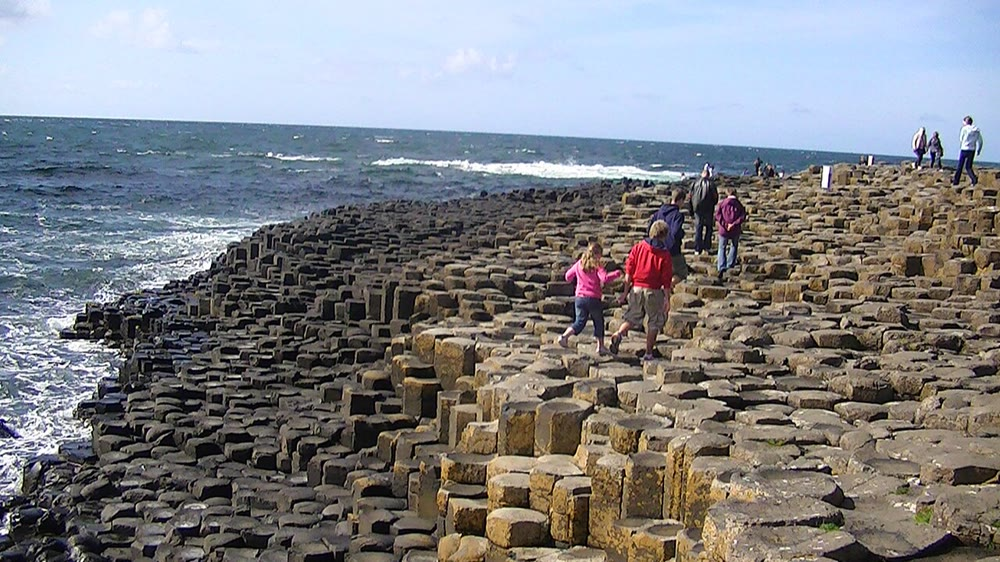
\includegraphics[height=4.3cm]{images/book2/g11-bishop-giants-causeway.jpg}\hspace{0.04\linewidth}%
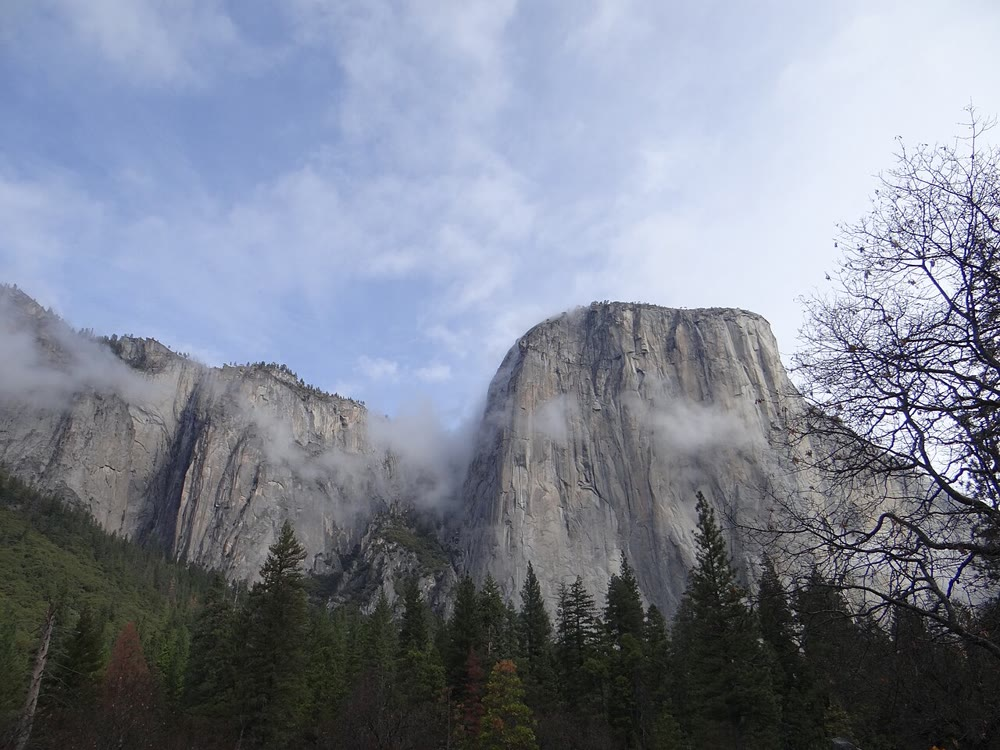
\includegraphics[height=4.3cm]{images/book2/g11-usgs-el-capitan.jpg}

{\small Kiri: tiang-tiang basalt Giant's Causeway, Irlandia Utara. Foto Adam
Bishop (CC~BY-SA~3.0). Kanan: El Capitan, Yosemite, California, dinding granit
yang tingginya sekitar \qty{900}{m}. Foto U.S. Geological Survey (CC0).}
\end{omfigure}
% ledger: photo:g11-giants-causeway, photo:g11-el-capitan

\begin{recall}
Magma adalah batuan cair di bawah permukaan; magma meletus sebagai lava, dengan
tenang atau secara eksplosif (Buku 1, kelas 7). Batuan beku adalah batuan yang
terbentuk ketika batuan cair mendingin dan menjadi padat (Buku 1, kelas 6).
Basalt adalah \omterm{def:g11:igneous-rocks:volcanic-plutonic}{batuan vulkanik} yang gelap, granit batuan terang yang tersusun
dari feldspar, kuarsa, dan mika (Buku 1, kelas 6). \omterm{def:g11:ocean-ridges:peridotite}{Peridotit} mantel meleleh
sebagian ketika naik di bawah punggungan, menghasilkan basalt dan \omterm{def:g11:ocean-ridges:gabbro}{gabro} \omterm{def:g11:ocean-ridges:oceanic-lithosphere}{kerak
samudra} (\cref{ch:g11:ocean-ridges}). \omterm{def:g11:minerals:rock-forming}{Silikat pembentuk batuan} adalah olivin,
piroksen, amfibol, mika, feldspar, dan kuarsa; feldspar terdiri atas feldspar
kalium dan plagioklas, sebuah deret dari yang kaya kalsium sampai yang kaya
natrium (\cref{ch:g11:minerals}). Kalor menyebar secara konduksi sejauh sekitar
$\sqrt{\kappa t}$ dalam waktu $t$, dengan $\kappa$ difusivitas termal
(\cref{ch:g11:subduction-zones}).
\end{recall}
% ledger: tulane:ridge-rocks, england:kelvin

\section{Batuan vulkanik dan batuan plutonik}

\begin{definition}[Batuan vulkanik; batuan plutonik]\label{def:g11:igneous-rocks:volcanic-plutonic}
Batuan beku, yang terbentuk oleh kristalisasi magma, disebut
\emph{batuan vulkanik}\index{batuan vulkanik}
(atau ekstrusif) bila magmanya membeku di permukaan Bumi, sebagai lava, dan
\emph{batuan plutonik}\index{batuan plutonik} (atau intrusif) bila magmanya
mengkristal di kedalaman, di dalam batuan lain.
\end{definition}
% ledger: tulane:magma-types

Perbedaannya tampak pada ukuran kristal. Sebuah kristal tumbuh dengan
menambahkan atom-atom yang diambil dari zat cair di sekitarnya, dan hal itu
memerlukan waktu. Di permukaan, lava cepat kehilangan kalornya ke udara atau ke
air: bahan yang dilontarkan ke udara atau ke air mendingin dalam hitungan detik,
aliran lava dalam beberapa hari sampai beberapa minggu. Jauh di bawah, batuan di
sekelilingnya panas dan magma kehilangan kalornya dengan lambat: \omterm{def:g11:igneous-rocks:intrusion}{intrusi} yang
dangkal mendingin dalam beberapa bulan sampai beberapa tahun, \omterm{def:g11:igneous-rocks:intrusion}{intrusi} besar yang
dalam mungkin memerlukan jutaan tahun. Pendinginan cepat menghasilkan banyak
kristal kecil, atau sama sekali tidak ada kristal; pendinginan lambat
menghasilkan kristal yang lebih sedikit tetapi jauh lebih besar.
% ledger: tulane:cooling-times, tulane:textures

\begin{definition}[Tekstur]\label{def:g11:igneous-rocks:texture}
Yang disebut \emph{tekstur}\index{tekstur (batuan)} sebuah batuan adalah ukuran,
bentuk, dan susunan butir-butirnya. Batuan beku bertekstur \emph{gelasan} bila
tidak mempunyai kristal, \emph{berbutir halus} bila kristal-kristalnya terlalu
kecil untuk dibedakan dengan mata telanjang, dan \emph{berbutir kasar} bila
semua kristalnya dapat dilihat.
\end{definition}
% ledger: tulane:textures

Lava yang terdinginkan mendadak sebelum satu kristal pun sempat tumbuh menjadi
kaca: obsidian, yang hitam dan gelasan, pecah dengan pecahan konkoidal seperti
pecahan botol. Basalt berbutir halus: di tangan, mineral-mineralnya tidak dapat
dikenali, dan bahkan dalam \omterm{def:g11:minerals:thin-section}{sayatan tipis} kristal-kristalnya kecil (basalt pada
\cref{ch:g11:minerals}). Granit, \omterm{def:g11:ocean-ridges:gabbro}{gabro}, dan \omterm{def:g11:igneous-rocks:rock-names}{diorit} berbutir kasar: setiap
butirnya tampak.
% ledger: photo:g11-obsidian, photo:g11-basalt, tulane:textures

\begin{definition}[Fenokris; porfiritik]\label{def:g11:igneous-rocks:porphyritic}
Yang disebut \emph{fenokris}\index{fenokris} adalah kristal besar yang terbenam
dalam massa kristal yang jauh lebih kecil atau dalam kaca, yaitu \emph{massa
dasar}. Batuan yang mempunyai fenokris disebut \emph{porfiritik}\index{porfiritik}.
\end{definition}
% ledger: tulane:textures

\omterm{def:g11:igneous-rocks:texture}{Tekstur} \omterm{def:g11:igneous-rocks:porphyritic}{porfiritik} merekam dua tahap pendinginan: mula-mula lambat, di
kedalaman, selagi \omterm{def:g11:igneous-rocks:porphyritic}{fenokris} tumbuh dalam magma yang sebagian besar masih cair;
lalu cepat, ketika magma naik dan meletus, atau disuntikkan ke dalam batuan yang
dingin, dan sisa zat cairnya membeku menjadi massa dasar.
% ledger: tulane:textures

\begin{omfigure}
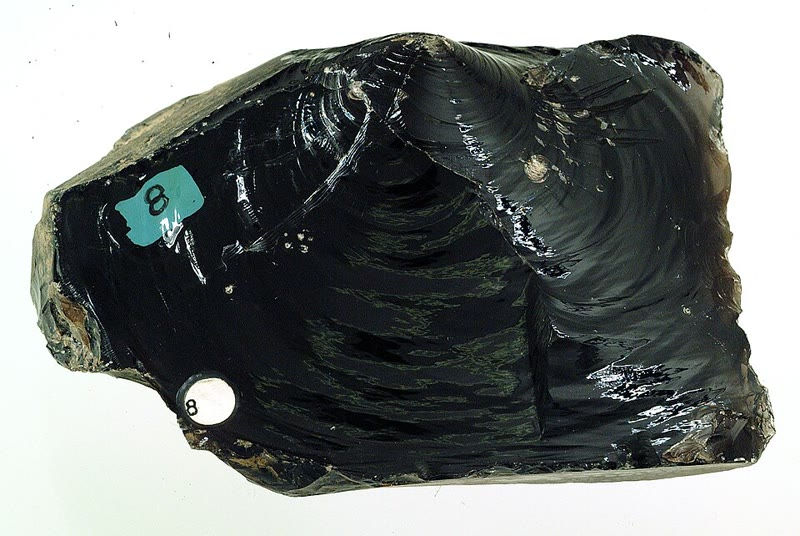
\includegraphics[height=2.75cm]{images/book2/g11-geodil-obsidian.jpg}\hfill
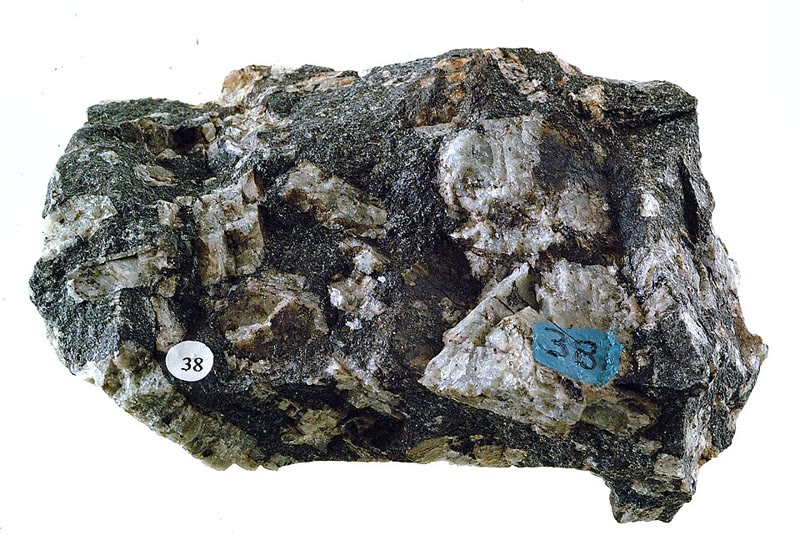
\includegraphics[height=2.75cm]{images/book2/g11-geodil-diabase-porphyry.jpg}\hfill
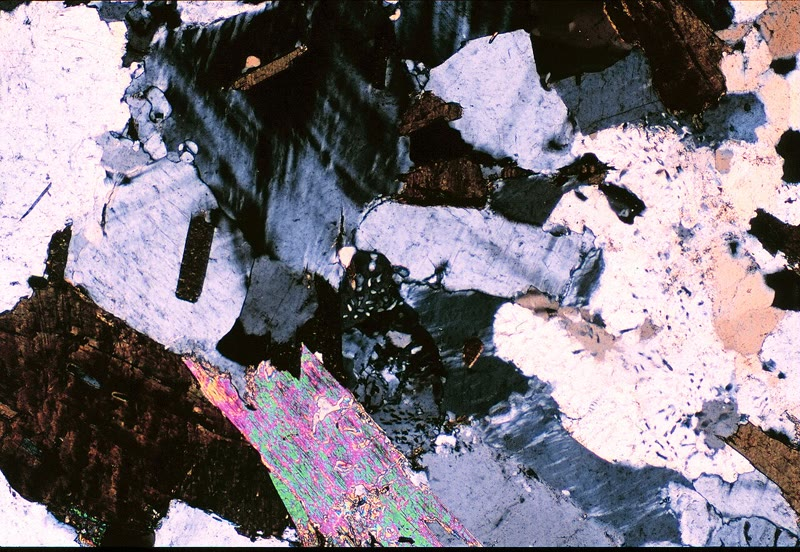
\includegraphics[height=2.75cm]{images/book2/g11-geodil-granite-xpl.jpg}\hfill
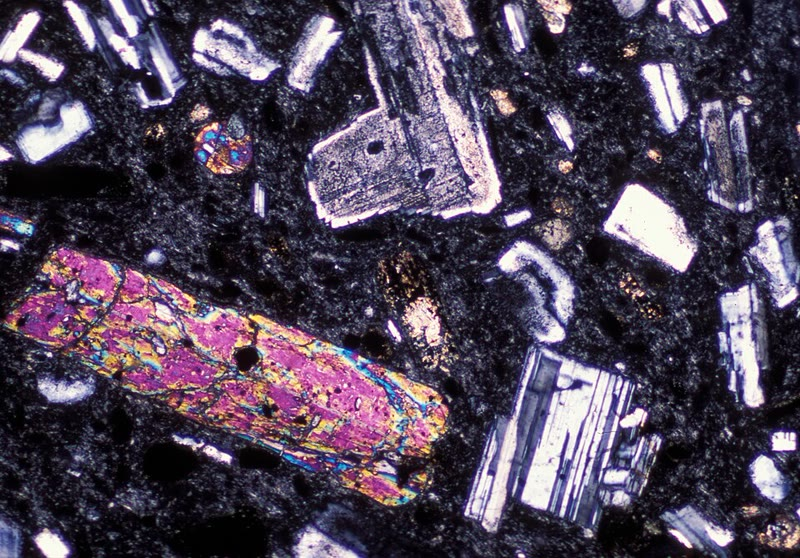
\includegraphics[height=2.75cm]{images/book2/g11-geodil-andesite-xpl.jpg}

{\small Dari kiri ke kanan: obsidian, sebuah kaca \omterm{def:g11:igneous-rocks:volcanic-plutonic}{vulkanik}, dengan pecahan
konkoidalnya yang melengkung (lebarnya \qty{9.5}{cm}); sebuah batuan \omterm{def:g11:igneous-rocks:porphyritic}{porfiritik},
dengan \omterm{def:g11:igneous-rocks:porphyritic}{fenokris} plagioklas berbentuk balok dalam massa dasar yang lebih halus
(\qty{9}{cm}); lalu dua \omterm{def:g11:minerals:thin-section}{sayatan tipis} di antara polarisator bersilang: sebuah
granit, yang semua butirnya besar dan saling mengunci --- biotit cokelat,
muskovit yang berwarna cerah, plagioklas yang bergaris-garis, kuarsa kelabu dan
putih; sebuah \omterm{def:g11:igneous-rocks:rock-names}{andesit}, dengan \omterm{def:g11:igneous-rocks:porphyritic}{fenokris} plagioklas dan amfibol dalam massa dasar
yang berbutir halus. Foto Twyla Baker, Mike Davis, dan Darla Sondrol,
Perpustakaan Citra Digital Geologi (GeoDIL) (CC0).}
\end{omfigure}
% ledger: photo:g11-obsidian, photo:g11-diabase-porphyry, photo:g11-granite-xpl, photo:g11-andesite-xpl

\section{Menamai batuan beku}

Kunci kedua sebuah batuan beku adalah kimianya, dan terutama kandungan
silikanya, \ce{SiO2}, yang pada magma-magma umum berkisar dari sekitar
\qty{45}{\percent} sampai sekitar \qty{75}{\percent} dari massanya.

\begin{definition}[Mafik; intermediet; felsik]\label{def:g11:igneous-rocks:felsic-mafic}
Sebuah magma, atau batuan yang dibentuknya, disebut \emph{mafik}\index{mafik}
bila mengandung sekitar \qty{45}{\percent} sampai \qty{55}{\percent} \ce{SiO2}
dan kaya akan besi, magnesium, dan kalsium; \emph{intermediet}\index{intermediet (batuan)}
bila kandungannya antara \qty{55}{\percent} dan \qty{65}{\percent}; \emph{felsik}\index{felsik}
bila mengandung sekitar \qty{65}{\percent} sampai \qty{75}{\percent} \ce{SiO2}
dan miskin besi, magnesium, dan kalsium tetapi kaya akan natrium dan kalium.
\end{definition}
% ledger: tulane:magma-types, earle:magma-oxides

Setiap jenis magma menghasilkan dua batuan, satu \omterm{def:g11:igneous-rocks:volcanic-plutonic}{vulkanik} dan berbutir halus,
satu \omterm{def:g11:igneous-rocks:volcanic-plutonic}{plutonik} dan berbutir kasar, dengan kimia yang sama. Basalt dan \omterm{def:g11:ocean-ridges:gabbro}{gabro}
adalah pasangan \omterm{def:g11:igneous-rocks:felsic-mafic}{mafik}, yang telah kita jumpai pada \omterm{def:g11:ocean-ridges:oceanic-lithosphere}{kerak samudra}; granit adalah
\omterm{def:g11:igneous-rocks:volcanic-plutonic}{batuan plutonik} \omterm{def:g11:igneous-rocks:felsic-mafic}{felsik}. Tiga nama melengkapi kumpulan ini.

\begin{definition}[Andesit; diorit; riolit]\label{def:g11:igneous-rocks:rock-names}
\emph{Andesit}\index{andesit} dan \emph{diorit}\index{diorit} adalah \omterm{def:g11:igneous-rocks:volcanic-plutonic}{batuan
vulkanik} dan \omterm{def:g11:igneous-rocks:volcanic-plutonic}{batuan plutonik} yang komposisinya \omterm{def:g11:igneous-rocks:felsic-mafic}{intermediet}, yang sebagian besar
tersusun dari plagioklas dengan amfibol atau piroksen. \emph{Riolit}\index{riolit}
adalah \omterm{def:g11:igneous-rocks:volcanic-plutonic}{batuan vulkanik} yang komposisinya \omterm{def:g11:igneous-rocks:felsic-mafic}{felsik}, padanan granit yang berbutir
halus.
\end{definition}
% ledger: tulane:magma-types, earle:bowen, photo:g11-andesite, photo:g11-diorite

\begin{omfigure}
\begin{tikzpicture}[font=\footnotesize, x=0.4cm]
  % columns: SiO2 45 to 75 % mapped to x = 45 to 75 (0.4 cm per %)
  \begin{scope}[xshift=-18cm]
  \fill[omLithBasalt!45] (45,0) rectangle (55,2.4);
  \fill[omLithBasalt!20] (55,0) rectangle (65,2.4);
  \fill[omLithGranite!45] (65,0) rectangle (75,2.4);
  \draw[black!60] (45,0) rectangle (75,2.4);
  \draw[black!60] (55,0) -- (55,2.4); \draw[black!60] (65,0) -- (65,2.4);
  \draw[black!60] (45,1.2) -- (75,1.2);
  \foreach \x/\a/\b in {50/basalt/gabro, 60/andesit/diorit, 70/riolit/granit}{
    \node[font=\small\bfseries, text height=1.6ex, text depth=0.3ex] at (\x,1.8) {\a};
    \node[font=\small\bfseries, text height=1.6ex, text depth=0.3ex] at (\x,0.6) {\b};}
  \node[anchor=east, align=right] at (44.4,1.8) {berbutir halus\\(vulkanik)};
  \node[anchor=east, align=right] at (44.4,0.6) {berbutir kasar\\(plutonik)};
  \node[anchor=south] at (50,2.45) {mafik};
  \node[anchor=south] at (60,2.45) {intermediet};
  \node[anchor=south] at (70,2.45) {felsik};
  % minerals (a drawing: where each mineral is common)
  \foreach \y/\a/\b/\m/\c in {-0.55/45.2/52/olivin/omLithBasalt!80!black,
      -1.15/45.2/61/piroksen/omLithBasalt!65!black,
      -1.75/52/69/amfibol/black!60,
      -2.35/57/74.8/biotit/black!75,
      -2.95/45.2/72/plagioklas/omDef!45,
      -3.55/63/74.8/feldspar kalium/omLithGranite!90!red,
      -4.15/64/74.8/kuarsa/black!20,
      -4.75/68/74.8/muskovit/black!35}{
    \fill[\c] (\a,\y) .. controls ({\a+1.2},{\y+0.22}) and ({\b-1.2},{\y+0.22}) .. (\b,\y)
              .. controls ({\b-1.2},{\y-0.22}) and ({\a+1.2},{\y-0.22}) .. (\a,\y) -- cycle;
    \node[anchor=east] at (44.4,\y) {\m};}
  \node[font=\scriptsize, text=black!75] at (50,-2.95) {kaya kalsium};
  \node[font=\scriptsize, text=omDef!80!black, anchor=west] at (72.3,-2.95) {kaya natrium};
  % SiO2 axis
  \draw[-{Stealth[length=4pt]}] (45,-5.35) -- (75.8,-5.35);
  \foreach \x in {45,50,...,75} {\draw (\x,-5.35) -- (\x,-5.45); \node[anchor=north] at (\x,-5.45) {\x};}
  \node[anchor=north] at (60,-5.85) {\ce{SiO2} (\unit{\percent} dari massa)};
  \draw[black!30, dashed] (55,0) -- (55,-5.35); \draw[black!30, dashed] (65,0) -- (65,-5.35);
  \end{scope}
\end{tikzpicture}

{\small Menamai batuan beku yang umum (sebuah gambar). Kolom: kandungan silika
magma; baris: batuan berbutir halus (\omterm{def:g11:igneous-rocks:volcanic-plutonic}{vulkanik}) dan berbutir kasar (\omterm{def:g11:igneous-rocks:volcanic-plutonic}{plutonik}).
Di bawah, tempat setiap mineral pembentuk batuan umum dijumpai: olivin dan
piroksen dalam batuan \omterm{def:g11:igneous-rocks:felsic-mafic}{mafik} bersama plagioklas yang kaya kalsium; amfibol dan
plagioklas dalam batuan \omterm{def:g11:igneous-rocks:felsic-mafic}{intermediet}; feldspar kalium, kuarsa, plagioklas yang
kaya natrium, dan mika dalam batuan \omterm{def:g11:igneous-rocks:felsic-mafic}{felsik}. Batas-batasnya berangsur.}
\end{omfigure}
% ledger: tulane:magma-types, earle:bowen, earle:magma-oxides, photo:g11-andesite, photo:g11-diorite, photo:g11-granite, nps:granite-minerals

\begin{method}[Menamai batuan beku]\label{met:g11:igneous-rocks:naming}
\begin{enumerate}
  \item Amati \omterm{def:g11:igneous-rocks:texture}{teksturnya}: gelasan, berbutir halus, atau berbutir kasar;
        \omterm{def:g11:igneous-rocks:porphyritic}{porfiritik} atau tidak. Berbutir halus atau gelasan berarti \omterm{def:g11:igneous-rocks:volcanic-plutonic}{vulkanik}
        (atau \omterm{def:g11:igneous-rocks:intrusion}{intrusi} kecil yang cepat mendingin); berbutir kasar berarti
        \omterm{def:g11:igneous-rocks:volcanic-plutonic}{plutonik}.
  \item Kenali mineral-mineral yang dapat dilihat
        (\cref{met:g11:minerals:identify}): kuarsa dan feldspar kalium
        menunjuk ke \omterm{def:g11:igneous-rocks:felsic-mafic}{felsik}, amfibol dengan plagioklas ke \omterm{def:g11:igneous-rocks:felsic-mafic}{intermediet}, olivin
        dan piroksen ke \omterm{def:g11:igneous-rocks:felsic-mafic}{mafik}. Pada batuan berbutir halus, gunakan
        \omterm{def:g11:igneous-rocks:porphyritic}{fenokrisnya}, warna massa dasarnya --- gelap untuk \omterm{def:g11:igneous-rocks:felsic-mafic}{mafik}, terang untuk
        \omterm{def:g11:igneous-rocks:felsic-mafic}{felsik} --- sebagai petunjuk, atau sebuah analisis kimia.
  \item Bacalah namanya pada perpotongan baris dan kolom diagram.
\end{enumerate}
\end{method}

\begin{example}[Dua basalt]
Sebuah batuan gelap dari aliran lava berbutir halus di seluruh bagiannya;
batuan lain, dari gunung api yang sama, memperlihatkan butir-butir olivin hijau
selebar beberapa milimeter dalam massa dasar yang gelap. Keduanya \omterm{def:g11:igneous-rocks:felsic-mafic}{mafik} dan
berbutir halus: keduanya basalt. Yang kedua adalah basalt \omterm{def:g11:igneous-rocks:porphyritic}{porfiritik}:
olivinnya tumbuh lebih dahulu, dengan lambat, di dalam magma di bawah gunung
api, sebelum lava meletus dan membeku di sekelilingnya.
\end{example}
% ledger: photo:g11-olivine, earle:bowen, tulane:textures

\begin{omfigure}
\makebox[0.32\linewidth]{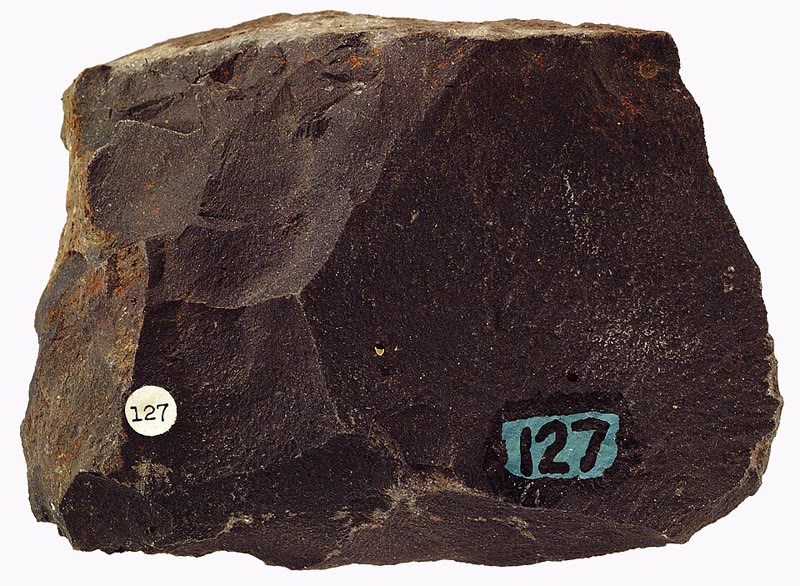
\includegraphics[height=2.9cm]{images/book2/g11-geodil-basalt.jpg}}\hfill
\makebox[0.32\linewidth]{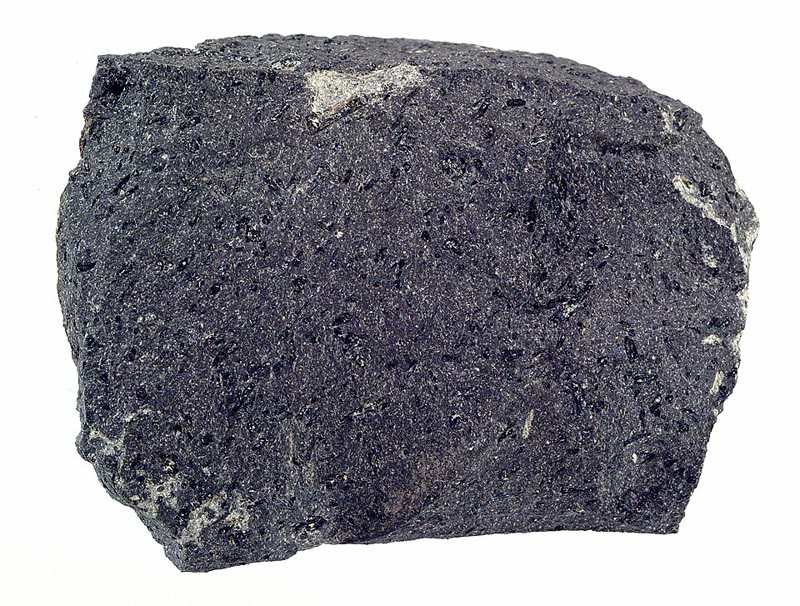
\includegraphics[height=2.9cm]{images/book2/g11-geodil-andesite.jpg}}\hfill
\makebox[0.32\linewidth]{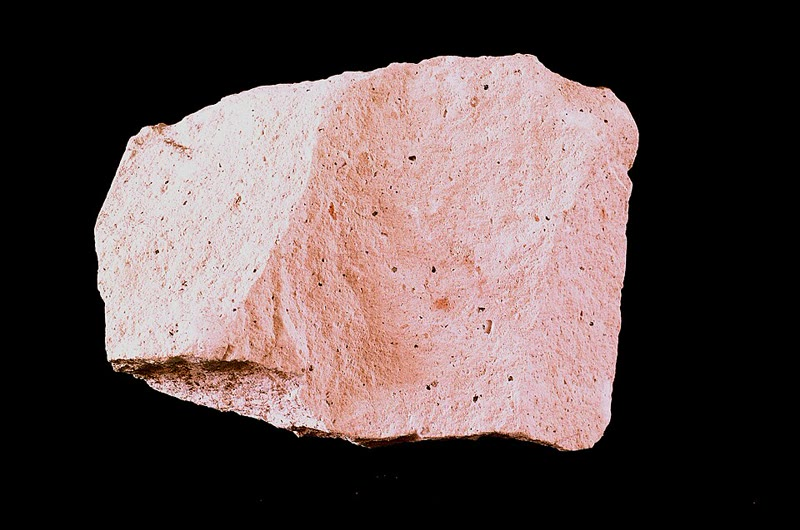
\includegraphics[height=2.9cm]{images/book2/g11-geodil-rhyolite.jpg}}

\smallskip
\makebox[0.32\linewidth]{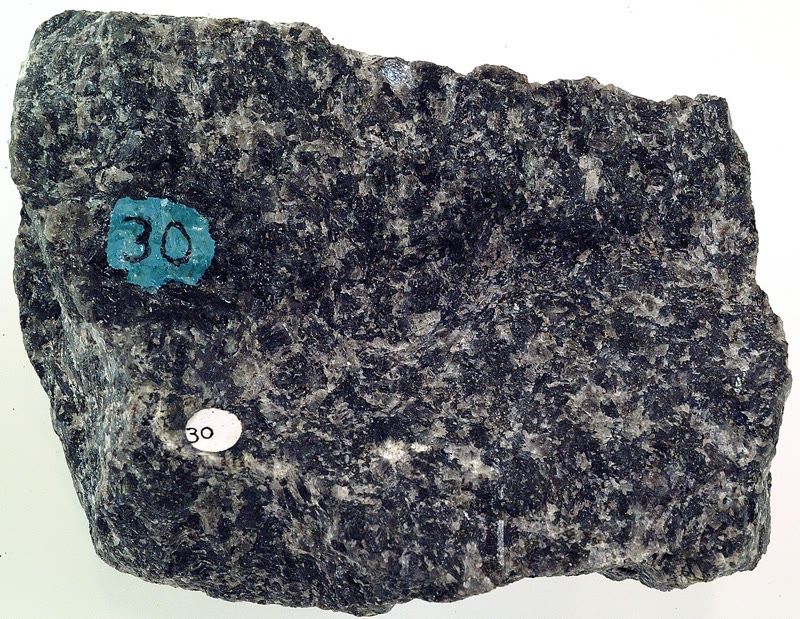
\includegraphics[height=2.9cm]{images/book2/g11-geodil-gabbro.jpg}}\hfill
\makebox[0.32\linewidth]{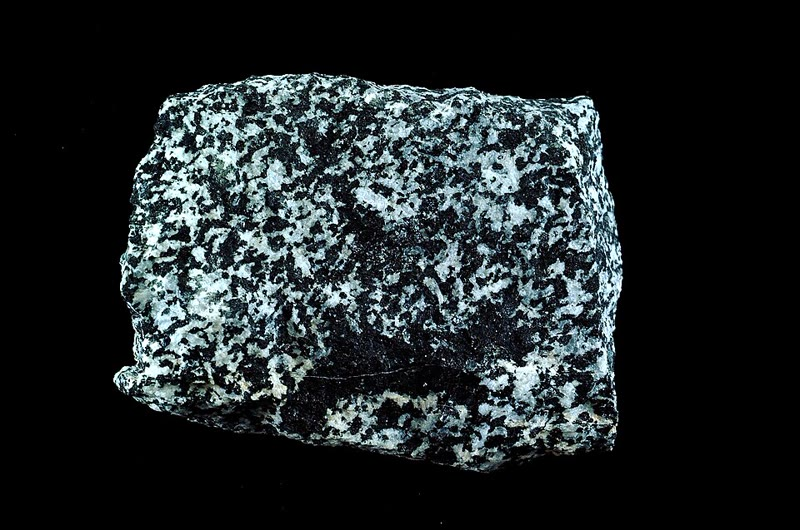
\includegraphics[height=2.9cm]{images/book2/g11-geodil-diorite.jpg}}\hfill
\makebox[0.32\linewidth]{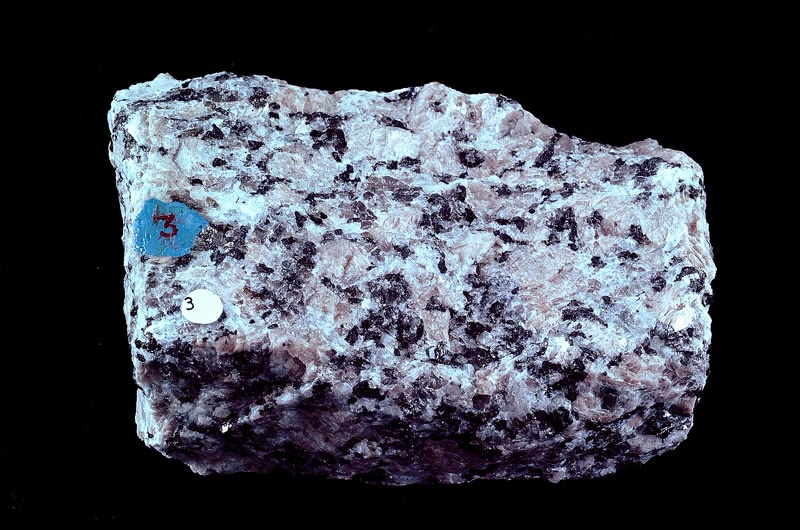
\includegraphics[height=2.9cm]{images/book2/g11-geodil-granite.jpg}}

{\small Tiga pasangan batuan beku, dari \omterm{def:g11:igneous-rocks:felsic-mafic}{mafik} ke \omterm{def:g11:igneous-rocks:felsic-mafic}{felsik} dari kiri ke kanan:
\omterm{def:g11:igneous-rocks:volcanic-plutonic}{vulkanik} di atas, \omterm{def:g11:igneous-rocks:volcanic-plutonic}{plutonik} di bawah. Atas: sebuah basalt berbutir halus; sebuah
\omterm{def:g11:igneous-rocks:rock-names}{andesit}, dengan kristal amfibol kecil dalam massa dasar yang berbutir halus
(sekitar \qty{10}{cm}); sebuah \omterm{def:g11:igneous-rocks:rock-names}{riolit} merah muda. Bawah: \omterm{def:g11:ocean-ridges:gabbro}{gabro} (\qty{9}{cm});
\omterm{def:g11:igneous-rocks:rock-names}{diorit}, dengan hornblende hitam dan plagioklas yang berkilap kaca
(\qty{10}{cm}); sebuah granit kasar dengan feldspar kalium besar yang berwarna
merah muda pucat, plagioklas kelabu, kuarsa, biotit, dan hornblende
(\qty{10}{cm}). Foto Nessa Eull, Twyla Baker, Joseph H.~Hartman, Darla Sondrol,
dan Dexter Perkins, Perpustakaan Citra Digital Geologi (GeoDIL) (CC0).}
\end{omfigure}
% ledger: photo:g11-basalt, photo:g11-andesite, photo:g11-rhyolite, photo:g11-gabbro, photo:g11-diorite, photo:g11-granite

\section{Urutan kristalisasi}

Magma tidak membeku pada satu suhu, seperti air. Mineral-mineralnya muncul satu
demi satu ketika magma mendingin, masing-masing dalam selang suhunya sendiri,
sehingga magma yang sedang mendingin dapat mengandung kristal dan masih sebagian
besar cair.

\begin{history}[Percobaan-percobaan Bowen]
Norman L.~Bowen (1887--1956) bergabung dengan Laboratorium Geofisika di Lembaga
Carnegie di Washington pada tahun 1912. Dengan bekerja terutama pada magma
basaltik, ia melelehkan batuan di dalam tungku, membiarkannya mendingin perlahan
sampai suhu yang dipilih sehingga sebagian mineral terbentuk, lalu
mendinginkannya secara mendadak, begitu cepat sehingga sisa zat cairnya menjadi
kaca. Di bawah mikroskop, kristal-kristal itu menunjukkan mineral mana yang
telah terbentuk di atas suhu tersebut. Dengan mengulanginya pada suhu yang makin
lama makin rendah, percobaan itu memberikan urutan munculnya mineral-mineral.
Bowen menerbitkan urutan ini sebagai sebuah deret reaksi pada tahun 1922 dan
bukunya \emph{The Evolution of the Igneous Rocks} pada tahun 1928.
\end{history}
% ledger: carnegie:bowen, earle:bowen

\begin{omfigure}
\begin{tikzpicture}[font=\footnotesize, box/.style={draw=black!60, rounded corners=2pt, fill=#1, minimum width=3.0cm, minimum height=0.62cm, align=center}]
  \node[box=omLithBasalt!45] (ol) at (0,0) {olivin};
  \node[box=omLithBasalt!35] (px) at (0,-1.1) {piroksen};
  \node[box=black!15] (am) at (0,-2.2) {amfibol};
  \node[box=black!25] (bi) at (0,-3.3) {biotit};
  \draw[-{Stealth[length=4pt]}, line width=0.8pt] (ol) -- (px);
  \draw[-{Stealth[length=4pt]}, line width=0.8pt] (px) -- (am);
  \draw[-{Stealth[length=4pt]}, line width=0.8pt] (am) -- (bi);
  \node[align=center, anchor=south] at (0,0.45) {\textbf{cabang diskontinu}\\setiap mineral bereaksi dengan zat cair\\menjadi mineral berikutnya};
  % continuous branch: a wedge from Ca-rich to Na-rich
  \fill[left color=omDef!55, right color=omDef!12, shading angle=180] (5.0,-0.9) -- (6.6,-0.9) -- (6.6,-3.5) -- (5.0,-3.5) -- cycle;
  \shade[top color=omDef!60, bottom color=omDef!10, draw=black!60, rounded corners=2pt] (4.3,-0.85) rectangle (7.3,-3.55);
  \node[align=center] at (5.8,-1.3) {plagioklas\\kaya kalsium};
  \node[align=center] at (5.8,-3.15) {plagioklas\\kaya natrium};
  \draw[-{Stealth[length=4pt]}, line width=0.8pt] (5.8,-1.65) -- (5.8,-2.7);
  \node[align=center, anchor=south] at (5.8,0.45) {\textbf{cabang kontinu}\\plagioklas berubah\\secara berangsur};
  % last minerals
  \node[box=omLithGranite!45, minimum width=7.6cm] (last) at (2.9,-4.75) {feldspar kalium, kuarsa, (muskovit)};
  \draw[-{Stealth[length=4pt]}, line width=0.8pt] (bi) -- (bi |- last.north);
  \draw[-{Stealth[length=4pt]}, line width=0.8pt] (5.8,-3.55) -- (5.8,-4.43);
  % temperature arrow
  \draw[-{Stealth[length=5pt]}, line width=1pt, omThm] (-2.6,0.3) -- (-2.6,-4.9);
  \node[anchor=east, align=right, text=omThm] at (-2.75,0.1) {pertama,\\\qtyrange{1200}{1300}{\degreeCelsius}};
  \node[anchor=east, align=right, text=omThm] at (-2.75,-4.7) {terakhir, sekitar\\\qtyrange{750}{800}{\degreeCelsius}};
  \node[anchor=east, align=right, text=omThm] at (-2.75,-2.3) {suhu\\turun};
\end{tikzpicture}

{\small Urutan mineral mengkristal dari magma yang sedang mendingin (deret
reaksi Bowen, sebuah gambar). Olivin terbentuk pertama; plagioklas mulai kurang
lebih pada titik ketika piroksen mulai, mula-mula kaya kalsium, lalu makin lama
makin kaya natrium. Feldspar kalium, kuarsa, dan kadang-kadang muskovit
terbentuk terakhir, dari sisa zat cair yang kaya silika.}
\end{omfigure}
% ledger: earle:bowen

Kata \emph{reaksi} itu penting. Olivin hanya stabil pada suhu tinggi: ketika
magma mendingin, kristal-kristal olivin bereaksi dengan silika dalam zat cair
dan berubah menjadi piroksen,
\[
  \ce{Mg2SiO4 + SiO2 -> 2 MgSiO3},
\]
dan begitu seterusnya menuruni cabang itu, selama silika masih ada dalam zat
cair. Di sepanjang cabang yang lain, kristal plagioklas terus tumbuh, tetapi
setiap lapisan barunya lebih kaya natrium daripada lapisan sebelumnya: kristal
plagioklas dapat berzona, dari inti yang kaya kalsium sampai tepi yang kaya
natrium, seperti \omterm{def:g11:igneous-rocks:porphyritic}{fenokris} plagioklas pada \omterm{def:g11:igneous-rocks:rock-names}{andesit} di atas.
% ledger: earle:bowen, photo:g11-andesite-xpl

Deret ini menjelaskan diagram tadi. Magma \omterm{def:g11:igneous-rocks:felsic-mafic}{mafik} kehabisan silika lebih awal:
magma itu mengkristalkan olivin, piroksen, dan plagioklas yang kaya kalsium, dan
menghasilkan \omterm{def:g11:ocean-ridges:gabbro}{gabro} bila mendingin perlahan di bawah tanah, basalt bila
mendingin cepat di permukaan. Hanya magma yang kaya silika yang berlanjut
sampai akhir deret dan membentuk feldspar kalium dan kuarsa: mineral-mineral
granit dan \omterm{def:g11:igneous-rocks:rock-names}{riolit}. Bagaimana sebuah magma mengubah komposisinya di sepanjang
jalan, ketika kristal-kristal awalnya terpisah dari zat cair, adalah pokok
bahasan tahun kedua perkuliahan.
% ledger: earle:bowen, tulane:bowen

\section{Intrusi}

Magma naik karena massa jenisnya lebih kecil daripada batuan di sekitarnya,
sambil memaksakan jalannya ke dalam rekahan dan melebarkannya. Sebagian besar
magma tidak pernah mencapai permukaan: magma itu mengkristal di dalam kerak
sebagai \omterm{def:g11:igneous-rocks:intrusion}{intrusi}, yang baru terlihat setelah erosi menyingkirkan batuan di
atasnya.
% ledger: tulane:intrusions

\begin{definition}[Retas; sill; pluton]\label{def:g11:igneous-rocks:intrusion}
Yang disebut \emph{intrusi}\index{intrusi} adalah tubuh batuan beku yang
mengkristal di dalam batuan lain. Yang disebut \emph{retas}\index{retas} adalah
lembaran batuan beku yang memotong lapisan atau struktur batuan yang
diterobosnya; yang disebut \emph{sill}\index{sill} adalah lembaran yang
terletak sejajar dengan lapisan-lapisan, di antara lapisan-lapisan itu. Yang
disebut \emph{pluton}\index{pluton} adalah intrusi besar dengan bentuk apa
pun, yang terbentuk di kedalaman; banyak pluton yang bergabung membentuk
sebuah batolit (\cref{ch:g12:subduction-magmatism}).
\end{definition}
% ledger: tulane:intrusions

Lebar \omterm{def:g11:igneous-rocks:intrusion}{retas} umumnya kurang dari \qty{20}{m} dan tebal \omterm{def:g11:igneous-rocks:intrusion}{sill} kurang dari
\qty{50}{m}; sebuah \omterm{def:g11:igneous-rocks:intrusion}{sill} biasanya dipasok oleh sebuah \omterm{def:g11:igneous-rocks:intrusion}{retas}. \omterm{def:g11:igneous-rocks:intrusion}{Retas} dan \omterm{def:g11:igneous-rocks:intrusion}{sill}
yang dangkal mendingin dengan cepat: keduanya berbutir halus, kadang-kadang
\omterm{def:g11:igneous-rocks:porphyritic}{porfiritik}. Berbatasan dengan batuan dingin yang diterobosnya, tepi-tepinya
mendingin paling cepat dan berbutir lebih halus lagi daripada bagian tengahnya:
sebuah \emph{tepi dingin}, tanda dari tubuh yang masih panas ketika menempati
tempatnya. Sierra Nevada di California, tempat Yosemite berada, adalah sebuah
batolit: batuan granitik yang massa jenisnya diukur pada \cref{ch:g11:minerals}
berasal dari sekitar dua ratus \omterm{def:g11:igneous-rocks:intrusion}{plutonnya}.
% ledger: tulane:intrusions, usgs91:sierra, photo:g11-el-capitan

\begin{omfigure}
\begin{tikzpicture}[font=\footnotesize, scale=0.9]
  % layered host rocks
  \fill[omLithSand] (0,0) rectangle (14,-1.0);
  \fill[omLithShale] (0,-1.0) rectangle (14,-2.0);
  \fill[omLithLime] (0,-2.0) rectangle (14,-3.0);
  \fill[omLithSand] (0,-3.0) rectangle (14,-4.0);
  \fill[omLithShale] (0,-4.0) rectangle (14,-6.4);
  \foreach \y in {-1,-2,-3,-4} \draw[black!35] (0,\y) -- (14,\y);
  % pluton
  \fill[omLithGranite, draw=black!60] (2.2,-6.4) .. controls (2.4,-4.6) and (3.6,-4.1) .. (5.5,-4.15)
     .. controls (7.4,-4.2) and (9.0,-4.5) .. (9.6,-6.4) -- cycle;
  % sill between the limestone and the shale, fed by the dyke
  \fill[omLithBasalt, draw=black!60] (7.3,-1.88) -- (12.6,-1.88) .. controls (12.9,-1.9) and (12.9,-2.1) .. (12.6,-2.12) -- (7.3,-2.12) -- cycle;
  % dyke from the pluton to the volcano
  \fill[omLithBasalt, draw=black!60] (7.0,-4.18) -- (7.3,-4.2) -- (7.3,0) -- (7.0,0) -- cycle;
  % a second dyke cutting across the layers, not reaching the surface
  \fill[omLithBasalt, draw=black!60] (3.9,-4.15) -- (4.15,-4.15) -- (2.95,-0.6) -- (2.75,-0.6) -- cycle;
  % volcano and lava flow
  \fill[black!65] (5.75,0) -- (7.15,1.35) -- (8.55,0) -- cycle;
  \fill[omLithBasalt!80!black] (8.4,0) -- (11.6,0) -- (11.6,0.1) .. controls (10.5,0.16) and (9.2,0.22) .. (8.3,0.15) -- cycle;
  \draw[black!70] (0,0) -- (5.75,0); \draw[black!70] (8.55,0) -- (14,0);
  % labels
  \node[anchor=south] at (7.15,1.4) {gunung api};
  \draw[black!60] (10.5,0.15) -- (11.2,0.8); \node[anchor=south west, inner sep=1pt] at (11.2,0.8) {aliran lava};
  \draw[black!60] (7.3,-0.5) -- (8.3,-0.5); \node[anchor=west, fill=omLithSand, inner sep=1pt] at (8.3,-0.5) {retas (memotong lapisan)};
  \draw[black!60] (11.0,-2.0) -- (11.0,-2.55); \node[anchor=north, fill=omLithLime, inner sep=1pt] at (11.0,-2.55) {sill (di antara lapisan)};
  \draw[black!60] (3.4,-2.5) -- (1.9,-2.5); \node[anchor=east, fill=omLithLime, inner sep=1pt] at (1.9,-2.5) {retas};
  \node[align=center] at (5.9,-5.5) {pluton};
  \node[anchor=east, fill=omLithShale, inner sep=1pt] at (13.85,-5.3) {batuan sedimen berlapis};
\end{tikzpicture}

{\small \omterm{def:g11:igneous-rocks:intrusion}{Intrusi} (sebuah gambar, tidak berskala). Sebuah \omterm{def:g11:igneous-rocks:intrusion}{pluton} mengkristal di
kedalaman; \omterm{def:g11:igneous-rocks:intrusion}{retas-retas} memotong lapisan batuan di atasnya, salah satunya
memasok sebuah gunung api; sebuah \omterm{def:g11:igneous-rocks:intrusion}{sill} menyebar di antara dua lapisan. Hanya
erosi batuan di atasnya yang menyingkapkan tubuh-tubuh ini di permukaan.}
\end{omfigure}
% ledger: tulane:intrusions

Berapa lama sebuah \omterm{def:g11:igneous-rocks:intrusion}{intrusi} mengkristal? Tinjaulah selembar magma --- sebuah
\omterm{def:g11:igneous-rocks:intrusion}{retas} atau sebuah \omterm{def:g11:igneous-rocks:intrusion}{sill} --- yang tebalnya $b$, yang kehilangan kalornya secara
konduksi ke batuan di kedua sisinya. Satu-satunya besaran yang menentukan
lajunya adalah tebal $b$, dalam meter, dan difusivitas termal $\kappa$, dalam
\unit{m^2/s}; satu-satunya waktu yang dapat disusun dari keduanya adalah $b^2/\kappa$.
% ledger: england:kelvin, delaney86:example

\begin{proposition}[Waktu pendinginan selembar magma]\label{prop:g11:igneous-rocks:cooling}
Selembar magma yang tebalnya $b$ dan yang mendingin secara konduksi membeku
dalam waktu
\[
  t = C\,\frac{b^2}{\kappa},
\]
dengan $\kappa$ difusivitas termal batuan dan $C$ sebuah bilangan yang
ditentukan oleh suhu magma dan suhu batuan di sekitarnya serta oleh kalor yang
dilepaskan ketika magma mengkristal. Menggandakan tebalnya mengalikan waktunya
dengan empat. (Diterima tanpa bukti; nilai $C$ berasal dari model yang
dihitung.)
\end{proposition}
% ledger: delaney86:properties, delaney86:example

Untuk magma basaltik yang menerobos pada \qty{1150}{\degreeCelsius} ke dalam
batuan bersuhu \qty{50}{\degreeCelsius}, yang mengkristal seluruhnya pada
\qty{950}{\degreeCelsius} dan melepaskan \qty{900}{MJ} kalor untuk setiap meter
kubik yang mengkristal, dengan $\kappa = \qty{1e-6}{m^2/s}$, model itu
memberikan $C \approx 0.21$. Selembar magma setebal \qty{2}{m} lalu membeku
dalam sekitar sepuluh hari, sebuah \omterm{def:g11:igneous-rocks:intrusion}{sill} setebal \qty{20}{m} dalam sekitar dua
setengah tahun, dan yang setebal \qty{100}{m} dalam sekitar enam puluh lima
tahun. Tanpa kalor kristalisasi, waktunya akan tiga kali lebih singkat: magma
yang sedang mengkristal menjaga dirinya tetap hangat.
% values (dyke_cooling.py): t2_day 9.55, t20_yr 2.61, t100_yr 65.3, latent_factor 2.94; C = 8.2475e7 s / 4e8 s = 0.206
% ledger: delaney86:example, delaney86:properties, england:kelvin

\begin{omfigure}
\begin{tikzpicture}
\begin{axis}[omrecord, name=times, width=0.45\linewidth, height=5.0cm, xmode=log, ymode=log,
  xmin=0.8, xmax=130, ymin=1e-3, ymax=200, xlabel={tebal lembaran (\unit{m})},
  ylabel={waktu sampai membeku (tahun)},
  legend style={font=\scriptsize, at={(0.5,-0.4)}, anchor=north, legend columns=2,
    /tikz/every even column/.append style={column sep=4pt}}]
% computed in figdata/grade-11/dyke_cooling.py; ledger: delaney86:*, england:kelvin
\addplot[omThm, line width=1pt, mark=*, mark size=1.4pt] table[x=b, y=t_yr] {figdata/out/grade-11-dyke_cooling-times.dat};
\addplot[omDef, line width=1pt, dashed, mark=o, mark size=1.4pt] table[x=b, y=t0_yr] {figdata/out/grade-11-dyke_cooling-times.dat};
\legend{dengan kalor kristalisasi, tanpa}
\end{axis}
\begin{axis}[omrecord, at={(times.east)}, anchor=west, xshift=1.6cm, width=0.45\linewidth, height=5.0cm,
  xmin=-28, xmax=28, ymin=0, ymax=1300, xlabel={jarak dari tengah sill (\unit{m})},
  ylabel={suhu (\unit{\degreeCelsius})},
  legend style={font=\scriptsize, at={(0.5,-0.4)}, anchor=north, legend columns=4,
    /tikz/every even column/.append style={column sep=4pt}}]
\fill[omLithBasalt!30] (axis cs:-10,0) rectangle (axis cs:10,1300);
\draw[black!50, dashed] (axis cs:-28,950) -- (axis cs:28,950);
\node[font=\scriptsize, anchor=south east, text=black!60] at (axis cs:27,955) {solidus};
\node[font=\scriptsize, anchor=north] at (axis cs:0,1290) {sill};
% computed in figdata/grade-11/dyke_cooling.py
\addplot[omProp, line width=0.9pt] table[x=x, y=T1] {figdata/out/grade-11-dyke_cooling-profiles.dat};
\addplot[omThm, line width=0.9pt] table[x=x, y=T2] {figdata/out/grade-11-dyke_cooling-profiles.dat};
\addplot[omDef, line width=0.9pt] table[x=x, y=T3] {figdata/out/grade-11-dyke_cooling-profiles.dat};
\addplot[black, line width=0.9pt] table[x=x, y=T4] {figdata/out/grade-11-dyke_cooling-profiles.dat};
\legend{30 hari, 6 bulan, 1 tahun, 2 tahun}
\end{axis}
\end{tikzpicture}

{\small Selembar magma basaltik yang mendingin secara konduksi (model yang
dihitung). Kiri: waktu yang diperlukannya untuk membeku, terhadap tebalnya, pada
sumbu logaritmik: sebuah garis lurus dengan kemiringan 2, sehingga waktunya
bertambah sebanding dengan kuadrat tebalnya. Kanan: suhu melintasi sebuah \omterm{def:g11:igneous-rocks:intrusion}{sill}
setebal \qty{20}{m} (diarsir), yang menerobos pada \qty{1150}{\degreeCelsius}
ke dalam batuan bersuhu \qty{50}{\degreeCelsius}. Tepi-tepinya langsung turun
di bawah solidus, bagian tengahnya baru setelah sekitar dua setengah tahun.}
\end{omfigure}
% values (dyke_cooling.py): profiles at 30, 180, 365, 730 days; contact about 690 degC (Delaney: 690)

Model itu juga memperlihatkan terbentuknya tepi dingin. Batuan pada bidang
kontak langsung melonjak ke sekitar \qty{690}{\degreeCelsius}, jauh di bawah
solidus: beberapa sentimeter pertama \omterm{def:g11:igneous-rocks:intrusion}{sill} itu membeku dalam satu hari,
sedangkan bagian tengahnya tetap cair selama bertahun-tahun. \omterm{def:g11:igneous-rocks:intrusion}{Intrusi} yang
sebenarnya lebih rumit --- sifat-sifat batuan berubah dengan suhu, air
bersirkulasi, \omterm{def:g11:igneous-rocks:intrusion}{pluton} yang dalam berada di dalam batuan yang sudah panas dan
dapat dipasok lagi berulang kali --- dan itulah sebabnya \omterm{def:g11:igneous-rocks:intrusion}{intrusi} besar yang
dalam memerlukan waktu jauh lebih lama untuk mendingin daripada yang
ditunjukkan oleh hukum itu, dengan batuan sekitar yang dingin.
% ledger: delaney86:example, tulane:cooling-times
% values (dyke_cooling.py): margin_day_20m 0.58 (cell 12.5 cm from the contact)

\section{Latihan}

\begin{exercise}[$\star$]\label{exo:g11:igneous-rocks:1}
Definisikan \omterm{def:g11:igneous-rocks:volcanic-plutonic}{batuan vulkanik} dan \omterm{def:g11:igneous-rocks:volcanic-plutonic}{batuan plutonik}. Sebutkan tiga pasangan \omterm{def:g11:igneous-rocks:volcanic-plutonic}{batuan
vulkanik} dan \omterm{def:g11:igneous-rocks:volcanic-plutonic}{plutonik} yang komposisinya sama, dari \omterm{def:g11:igneous-rocks:felsic-mafic}{mafik} ke \omterm{def:g11:igneous-rocks:felsic-mafic}{felsik}.
\end{exercise}

\begin{exercise}[$\star$]\label{exo:g11:igneous-rocks:2}
Pasangkan setiap batuan dengan \omterm{def:g11:igneous-rocks:texture}{teksturnya} --- gelasan, berbutir halus, berbutir
kasar, \omterm{def:g11:igneous-rocks:porphyritic}{porfiritik}: (1) obsidian; (2) granit; (3) basalt dengan kristal olivin
hijau selebar beberapa milimeter dalam massa dasar yang gelap; (4) basalt yang
tidak satu mineral pun dapat dilihat di dalamnya.
\end{exercise}

\begin{exercise}[$\star$]\label{exo:g11:igneous-rocks:3}
Tiga magma mengandung \qty{48}{\percent}, \qty{60}{\percent}, dan
\qty{72}{\percent} \ce{SiO2}. Golongkan masing-masing, dan sebutkan batuan yang
dihasilkan masing-masing bila mendingin perlahan di kedalaman.
\end{exercise}

\begin{exercise}[$\star$]\label{exo:g11:igneous-rocks:4}
Definisikan \omterm{def:g11:igneous-rocks:intrusion}{retas}, \omterm{def:g11:igneous-rocks:intrusion}{sill}, dan \omterm{def:g11:igneous-rocks:intrusion}{pluton}. Pada gambar \omterm{def:g11:igneous-rocks:intrusion}{intrusi} dalam bab ini, tubuh
manakah yang memasok gunung api?
\end{exercise}

\begin{exercise}[$\star$]\label{exo:g11:igneous-rocks:5}
Dalam deret reaksi Bowen, mineral manakah yang terbentuk pertama, dan mineral
manakah yang terbentuk terakhir? Bagaimana plagioklas berubah ketika magma
mendingin?
\end{exercise}

\begin{exercise}[$\star\star$]\label{exo:g11:igneous-rocks:6}
Dua batuan dianalisis (persen massa). Batuan A: \ce{SiO2} 74, \ce{Al2O3}
14, \ce{FeO} 3, \ce{CaO} 3, \ce{MgO} 0.5, \ce{Na2O} 5, \ce{K2O} 4. Batuan B:
\ce{SiO2} 47, \ce{Al2O3} 14, \ce{FeO} 8, \ce{CaO} 10, \ce{MgO} 8, \ce{Na2O}
1, \ce{K2O} 2. (1) Golongkan masing-masing. (2) Periksa jawabanmu dengan
oksida-oksida lainnya. (3) Batuan A berbutir halus: sebutkan namanya. Batuan B
berbutir kasar: sebutkan namanya.
\end{exercise}

\begin{exercise}[$\star\star$]\label{exo:g11:igneous-rocks:7}
Sebuah \omterm{def:g11:igneous-rocks:intrusion}{retas} setebal \qty{2}{m} membeku dalam sekitar sepuluh hari. Dengan
proposisi tentang waktu pendinginan, berapa lama waktu yang diperlukan sebuah
\omterm{def:g11:igneous-rocks:intrusion}{retas} dari magma yang sama bila tebalnya \qty{1}{m}? Sebuah \omterm{def:g11:igneous-rocks:intrusion}{sill} setebal
\qty{20}{m}? Yang setebal \qty{200}{m}?
\end{exercise}

\begin{exercise}[$\star\star$]\label{exo:g11:igneous-rocks:8}
(1) Tunjukkan bahwa $b^2/\kappa$ adalah sebuah waktu. (2) Hitung nilainya untuk
$b = \qty{20}{m}$ dan $\kappa = \qty{1e-6}{m^2/s}$, dalam detik dan dalam tahun
($\num{1}\text{ tahun} \approx \qty{3.16e7}{s}$). (3) Dengan $C = 0.21$, berapa
lama \omterm{def:g11:igneous-rocks:intrusion}{sill} itu membeku?
\end{exercise}

\begin{exercise}[$\star\star$]\label{exo:g11:igneous-rocks:9}
Sebuah batuan memperlihatkan kristal-kristal plagioklas berbentuk balok yang
panjangnya sekitar satu sentimeter dalam massa dasar yang butir-butirnya tidak
dapat dilihat. Jelaskan \omterm{def:g11:igneous-rocks:texture}{teksturnya}, dan ceritakan kisah pendinginannya dalam
dua tahap.
\end{exercise}

\begin{exercise}[$\star\star$]\label{exo:g11:igneous-rocks:10}
Olivin bereaksi dengan silika dalam zat cair: $\ce{Mg2SiO4 + SiO2 -> 2
MgSiO3}$. (1) Periksa bahwa persamaan itu setara. (2) Dengan massa molar
\qty{140.7}{g/mol} (\ce{Mg2SiO4}) dan \qty{60.1}{g/mol} (\ce{SiO2}), berapa
massa silika yang diambil \qty{1}{kg} olivin dari zat cair? (3) Mengapa magma
yang miskin silika mempertahankan olivinnya?
\end{exercise}

\begin{exercise}[$\star\star$]\label{exo:g11:igneous-rocks:11}
Sebuah \omterm{def:g11:igneous-rocks:intrusion}{sill} setebal \qty{20}{m} dengan luas \qty{1}{m^2} mendingin dari
\qty{1150}{\degreeCelsius} ke \qty{50}{\degreeCelsius}. (1) Kapasitas kalornya
\qty{2.5}{MJ} per meter kubik dan per derajat: berapa kalor yang hilang
karena pendinginan itu? (2) \omterm{def:g11:igneous-rocks:intrusion}{Sill} itu juga melepaskan \qty{900}{MJ} per meter
kubik ketika mengkristal: berapa kalor itu? (3) Bandingkan keduanya.
\end{exercise}

\begin{exercise}[$\star\star\star$]\label{exo:g11:igneous-rocks:12}
Dalam model yang dihitung untuk sebuah \omterm{def:g11:igneous-rocks:intrusion}{sill} setebal \qty{20}{m}, batuan yang
berjarak \qty{12.5}{cm} dari bidang kontak turun di bawah solidus setelah
sekitar \num{0.6}~hari, batuan yang berjarak \qty{5}{m} dari bidang kontak
setelah sekitar 545 hari, dan bagian tengahnya setelah sekitar 950 hari. (1) Di
bagian mana dalam \omterm{def:g11:igneous-rocks:intrusion}{sill} itu kamu perkirakan kristal-kristal terkecil, dan di
mana yang terbesar? (2) Apakah laju pertumbuhan lapisan padat itu tetap?
(3) Mengapa \omterm{def:g11:igneous-rocks:intrusion}{sill} itu berbutir halus bahkan di bagian tengahnya, dibandingkan
dengan granit?
\end{exercise}

\begin{exercise}[$\star\star\star$]\label{exo:g11:igneous-rocks:13}
Sebuah \omterm{def:g11:igneous-rocks:intrusion}{pluton} tebalnya \qty{2}{km}. (1) Dengan proposisi itu dan \omterm{def:g11:igneous-rocks:intrusion}{sill} setebal
\qty{20}{m} (sekitar 2.6 tahun), perkirakan waktu pendinginannya. (2) \omterm{def:g11:igneous-rocks:intrusion}{Intrusi}
besar yang dalam diketahui memerlukan waktu sampai jutaan tahun untuk mendingin.
Berikan dua alasan mengapa hukum yang sederhana itu meremehkan waktunya.
\end{exercise}

\begin{exercise}[$\star\star\star$]\label{exo:g11:igneous-rocks:14}
Magma \omterm{def:g11:igneous-rocks:felsic-mafic}{felsik} meletus pada sekitar \qtyrange{650}{800}{\degreeCelsius}, magma
\omterm{def:g11:igneous-rocks:felsic-mafic}{mafik} pada sekitar \qtyrange{1000}{1200}{\degreeCelsius}. Dengan deret reaksi
Bowen, jelaskan mengapa granit mengandung feldspar kalium, kuarsa, dan
plagioklas yang kaya natrium, tanpa olivin, sedangkan \omterm{def:g11:ocean-ridges:gabbro}{gabro} mengandung olivin,
piroksen, dan plagioklas yang kaya kalsium, tanpa kuarsa.
\end{exercise}

\begin{exercise}[$\star\star\star$]\label{exo:g11:igneous-rocks:15}
Bahan yang dilontarkan ke udara mendingin dalam hitungan detik, aliran lava
dalam beberapa hari sampai beberapa minggu, \omterm{def:g11:igneous-rocks:intrusion}{intrusi} dangkal dalam beberapa
bulan sampai beberapa tahun. (1) Dengan proposisi itu, berapa tebal lembaran
yang membeku dalam sekitar satu hari? (2) Sebuah aliran lava setebal
\qty{5}{m} membeku dalam sekitar satu bulan: apakah hal itu sesuai dengan hukum
untuk lembaran yang didinginkan pada kedua sisinya? (3) \omterm{def:g11:igneous-rocks:texture}{Tekstur} mana yang kamu
perkirakan pada masing-masing kasus?
\end{exercise}

\section{Soal: Sebuah Sill dan Kristal-Kristalnya}

\begin{problem}[{Soal akhir pekan --- berapa lama sebuah sill membeku}]
\label{pb:g11:igneous-rocks:1}
% values (dyke_cooling.py): t20_yr 2.61, margin_day_20m 0.58, t2_day 9.55, contact ~690 degC;
% C = 0.206; ledger delaney86:*, tulane:*, earle:*
Di dinding sebuah lembah, selembar batuan beku gelap setebal \qty{20}{m}
terletak di antara dua lapisan batu pasir, sejajar dengan keduanya. Contoh-contoh
diambil dari tepinya sampai ke bagian tengahnya. Pada bidang kontak batuannya
sangat berbutir halus, hampir gelasan; \qty{1}{m} ke dalam, kristal-kristalnya
berukuran sekitar \qty{0.1}{mm}; di bagian tengah, sekitar \qty{1}{mm}, dan
plagioklas serta piroksen baru dapat dibedakan dengan kaca pembesar.

\medskip
\noindent\textbf{Bagian I --- Tekstur.}
\begin{enumerate}
  \item Apakah lembaran itu \omterm{def:g11:igneous-rocks:intrusion}{retas} atau \omterm{def:g11:igneous-rocks:intrusion}{sill}? Mengapa?
  \item Jelaskan \omterm{def:g11:igneous-rocks:texture}{tekstur} pada bidang kontak dan di bagian tengah.
  \item Mengapa batuan itu paling halus butirnya pada bidang kontak?
  \item Apa nama tepi berbutir halus ini, dan apa yang dibuktikannya tentang
        suhu lembaran itu ketika menempati tempatnya?
  \item Lembaran itu dipasok dari bawah oleh selembar batuan yang sama yang
        tegak, setebal \qty{2}{m}, yang memotong batu pasir. Apakah itu?
\end{enumerate}

\medskip
\noindent\textbf{Bagian II --- Menamai batuan.}
\begin{enumerate}[resume]
  \item Sebuah analisis memberikan \qty{49}{\percent} \ce{SiO2}, \qty{10}{\percent}
        \ce{FeO}, \qty{7}{\percent} \ce{MgO}, dan \qty{10}{\percent}
        \ce{CaO}. Apakah magma itu \omterm{def:g11:igneous-rocks:felsic-mafic}{mafik}, \omterm{def:g11:igneous-rocks:felsic-mafic}{intermediet}, atau \omterm{def:g11:igneous-rocks:felsic-mafic}{felsik}?
  \item Mineral-mineral apa yang kamu perkirakan, menurut deret Bowen?
  \item Nama mana yang cocok untuk batuan pada bidang kontak? \omterm{def:g11:igneous-rocks:volcanic-plutonic}{Batuan plutonik}
        mana yang komposisinya sama?
  \item Mengapa satu tubuh magma dapat menghasilkan batuan dengan \omterm{def:g11:igneous-rocks:texture}{tekstur} yang
        berbeda-beda?
  \item Dalam urutan apa olivin, piroksen, dan plagioklas mulai mengkristal?
\end{enumerate}

\medskip
\noindent\textbf{Bagian III --- Waktu pendinginan.}
\begin{enumerate}[resume]
  \item Hitung $b^2/\kappa$ untuk \omterm{def:g11:igneous-rocks:intrusion}{sill} itu, dengan $\kappa = \qty{1e-6}{m^2/s}$,
        dalam detik.
  \item Model itu memberikan $C = 0.206$. Hitung waktu yang diperlukan \omterm{def:g11:igneous-rocks:intrusion}{sill} itu untuk membeku, dalam
        detik, lalu dalam tahun ($\num{1}\text{ tahun} \approx \qty{3.16e7}{s}$).
  \item Berapa lama waktu yang diperlukan lembaran pemasoknya, yang setebal
        \qty{2}{m}?
  \item Tanpa kalor kristalisasi, $C$ akan sekitar $0.07$.
        Berapa lama \omterm{def:g11:igneous-rocks:intrusion}{sill} itu akan membeku? Mengapa kristalisasi memperlambat
        pendinginan?
  \item Model itu memberikan sekitar \num{0.6}~hari untuk batuan yang berjarak
        \qty{12.5}{cm} dari bidang kontak. Berapa kali lebih cepat batuan itu
        membeku daripada bagian tengahnya?
\end{enumerate}

\medskip
\noindent\textbf{Bagian IV --- Apa yang diceritakan kristal-kristal itu.}
\begin{enumerate}[resume]
  \item Aliran lava mendingin dalam beberapa hari sampai beberapa minggu,
        \omterm{def:g11:igneous-rocks:intrusion}{intrusi} dangkal dalam beberapa bulan sampai beberapa tahun. Di mana
        tempat \omterm{def:g11:igneous-rocks:intrusion}{sill} itu?
  \item Granit dengan kristal berukuran satu sentimeter atau lebih mendingin
        jauh lebih lambat. Dengan hukum itu, perkirakan tebal lembaran yang
        akan memerlukan waktu seribu kali lebih lama daripada \omterm{def:g11:igneous-rocks:intrusion}{sill} itu.
  \item Mengapa tubuh seperti itu pasti terbentuk jauh di dalam kerak?
  \item \omterm{def:g11:igneous-rocks:intrusion}{Sill} itu kini terlihat di permukaan. Apa yang pasti telah terjadi pada
        batuan yang dahulu berada di atasnya?
  \item Simpulkan: berapa lama \omterm{def:g11:igneous-rocks:intrusion}{sill} itu membeku?
\end{enumerate}
\end{problem}
